Software synthesis for multicores is effective because we use \acp{MoC} that expose concurrency.
The most natural way of leveraging the exposed concurrency is parallelism. 
When writing code using explicit models in the dataflow family, like \ac{KPN} or \ac{SDF}, the concurrency also becomes explicit.
However, in an implicit language like Ohua, we need to be careful to consider stateful computation when extracting concurrency.

Ohua uses a special operator, \texttt{smap}, to derive concurrency from stateful computation.
The principle behind \texttt{smap} is that it extends the higher-order \texttt{map} function to consider the state of the function it maps.
This adds a dependency between multiple executions of the same (stateful) function.
For a single function mapped over a collection, this principle exposes no concurrency. There is none, in general.
However, when we compose multiple functions in a \texttt{map}, we get a different picture.

Consider three (stateful) functions, $f: a \rightarrow b$ and $g : b \rightarrow c$, $h : c \rightarrow d$ with respective states $S_a, S_b$ and $S_c$, which we thus model as functions: 
\begin{align*}
sf : a \times S_f \rightarrow b \times S_f, sg : b \times S_g \rightarrow c \times S_g, sh : c \times S_h \rightarrow d \times S_h
\end{align*}

We use the prefix \texttt{s} to distinguish the stateful version of the function (with the state dependencies explicit).
Then, we get the dependency graph for the execution of the (Haskell) expression \texttt{map (f.g.h) inputs} as depicted in Figure~\ref{fig:smap_state}

\begin{figure}[h]
	\centering
	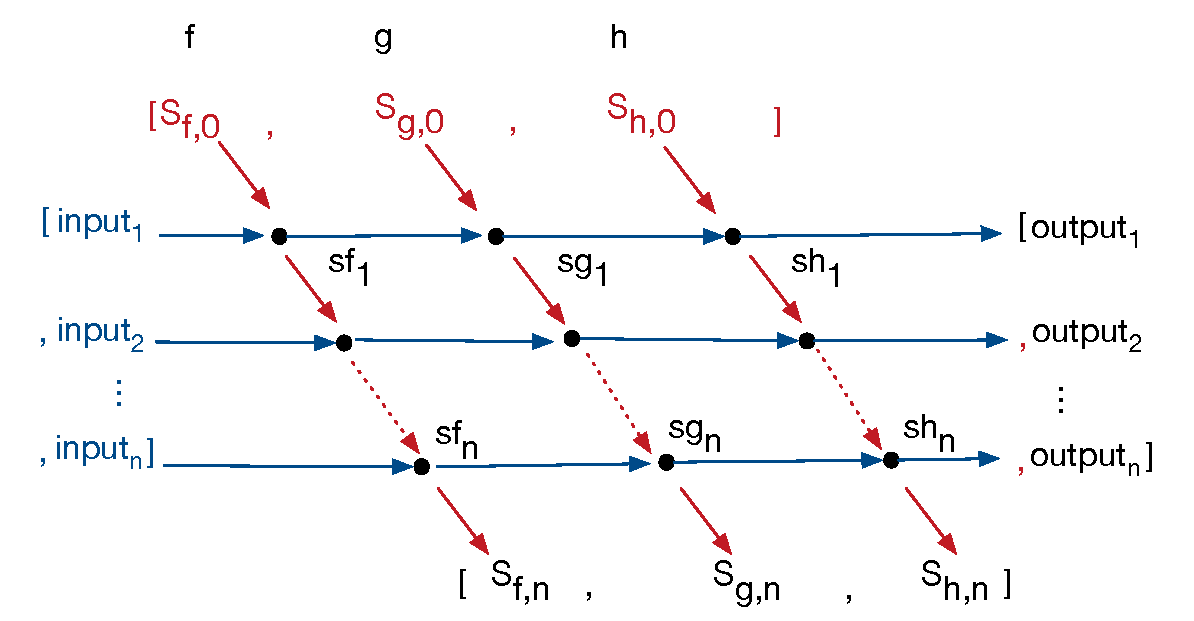
\includegraphics[scale=0.5]{figures/smap_state.pdf}
	\caption{ Dependencies of \mintinline{Haskell}{(map (f . g . h) inputs)}. Adapted from Figure~5 in~\cite{ertel_haskell19}}
	\label{fig:smap_state}
	%	\vspace{-1mm}
\end{figure}

The pattern we see in Figure~\ref{fig:smap_state} is very similar to the higher-order function \texttt{scan} on the state.
Intuitively, if we consider the function \texttt{sf'} that only returns the state of \texttt{sf}, then the state $S_{f,i} := (S_f)_i$ corresponds to the $i$-th value of the expression \texttt{scanl sf' $S_{f,_0}$ input}.
Threading the state around \texttt{f} explicitly can be achieved with the functional pattern known as a monad, in a fashion similar to the state monad in Haskell. 
Two different concrete implementations of this principle in Haskell are discussed in~\cite{ertel_haskell19}. These implementations are beyond the scope of this thesis.
The result of this monadic composition of state threads, however, is that we can write virtually the same expression as above in a monadic composition:

\begin{minted}[]{Haskell}
smap (f >=> g >=> h) inputs
\end{minted}

The \texttt{>=>} operator is the monadic equivalent of function composition, with the \texttt{.} (dot) operator. This yields the dependencies explicitly.
Similarly, these state threads and their composition can be formalized using category theory~\cite{ertel_haskellsup19}.
This formalization is rather technical. We will only sketch it here.

Let $\mathcal{C}$ be a Cartesian closed category, which is a technical condition that in a model-theoretic interpretation of categories corresponds to the typed $\lambda$ calculus~\cite{huet1985cartesian}.
We can think of $\mathcal{C}$ as the values and functions of the language, like the category of Haskell types $\operatorname{Hask}$\footnote{Note that this might not, strictly speaking, be a category. See \url{http://math.andrej.com/2016/08/06/hask-is-not-a-category/}}.
A Cartesian closed category has a terminal object $\bot \in \operatorname{Obj}(\mathcal{C})$, and any two objects $B,C \in \operatorname{Obj}(\mathcal{C})$ have a product $B \times C$ and an exponential $B^Y$.
These constructions are defined via universal properties in commutative diagrams and are rather technical.
We will omit the precise definitions here for space reasons.
It suffices to say they correspond with the known constructions, e.g. the product is the Cartesian product in the category $\operatorname{Set}$ of sets. 

The main idea of formalizing and dealing with state threads is to index them.
We do this through a (countable) index set $N \subseteq \mathbb{N}$, which for practical purposes we can also think of as being finite.
We ``split'' the state into local states which correspond to the indices in $N$. Formally, let $S_i \in \operatorname{Obj}(\mathcal{C}), i \in N$ be pairwise distinct (i.e. $i \neq j \Rightarrow S_i \neq S_j$).
We define for $I \subseteq N$ the \emph{state object} $S_I = \times_{i \in I} S_i$ as the product of the $S_i$ for all $i \in I$. If $I = N$, we call the state object $S_N$ the \emph{global state}.
The individual states $S_i := S_{\{i\}}$ for $i \in N$ we call fundamental states. We thus formally define a \emph{state thread}\index{state thread} as a morphism:
\begin{align*}
  f : (a \times S_I) \rightarrow (b \times S_I), \text{ for an } I \subseteq N
\end{align*}

This definition formalizes the intuition behind Equation~\ref{eqn:state_thread}. 
It is justified by Lemma~\ref{lem:state_thread_subcategory}.

\begin{lem}[Lemma~1.3 of \cite{ertel_haskellsup19}]
\label{lem:state_thread_subcategory}
The following define the objects and morphisms of a subcategory $\mathcal{S}$ of $\mathcal{C}$,
\begin{align}
	& \operatorname{Obj}({\mathcal{S}}) = \left\{ a\times s_I \mid
		a\in\operatorname{Obj}({\mathcal{C}}),
	 	I\subseteq N \right\} \,, \\
	& \operatorname{Morph}({\mathcal{S}}) = \left\{ f : (a\times s_I) \rightarrow (b\times s_I) \mid
		f\in\operatorname{Morph}({\mathcal{C}}),
		I\subseteq N \right\} \,.
\end{align}%
\begin{proof}
Since $\mathcal{C}$ is a category, and as such the composition of morphisms behaves as required, it suffices to show that morphisms respect the structure of the subcategory.
It is clear that $\operatorname{id}_{a\times s_I} \in \operatorname{Morph}(\mathcal{S})$ for every $a \in \operatorname{Obj}(\mathcal{C}), I \subseteq N$, since $\operatorname{id}_a \in \operatorname{Morph}(\mathcal{C})$.
Let $f,g \in \operatorname{Morph}(\mathcal{S})$ with such that $g \circ f$ is defined in $\mathcal{C}$.
Then it has to hold that there are $a,b$ and $c \in \operatorname{Obj}(C)$ as well as $I \subseteq N$, such that $f : (a \times S_I) \rightarrow (b \times S_I)$ and $g : (b \times S_I) \rightarrow (c \times S_I)$,
since $g \circ f$ is defined in $\mathcal{C}$. But then $g \circ f : (a \times S_I) \rightarrow (c \times S_I)$ is in $\operatorname{Morph}(\mathcal{S})$ by definition of $\mathcal{S}$.
\end{proof}
\end{lem}%

Intuitively, we think of a state thread $f : (a \times S_I) \rightarrow (b \times S_I)$ as operating only on the state object $S_I$, which is a part of the global state $S_N$.
As can be seen from the proof of Lemma~\ref{lem:state_thread_subcategory}, state threads compose when they have the same state objects $S_I$.
The goal of the formalism is to be able to extend this composition to arbitrary $I,J \subseteq N$.
In particular, this gives us a framework to reason about the dependencies of state threads.
Indeed, if $I \cap J = \emptyset$, then the state threads $f : (a \times S_I) \rightarrow (b \times S_I)$ and $g : (c \times S_J) \rightarrow (d \times S_J)$ are concurrent.

The definition of a general composition of state threads is, again, somewhat technical. We will only sketch it here: Given a state thread $f : (a \times S_I) \rightarrow (b \times S_I)$,
the idea is to define an extension $f* : (a \times S_N) \rightarrow (b \times S_N)$ which acts as an identity on $a \times S_{N \setminus I}$. 
By using a technical construction, this extension can be made such that the information of the $I$ is kept, while allowing a well-defined composition of state threads.
In this way, the resulting category allows us to elevate arbitrary computations in $\mathcal{C}$ to state threads in a fashion that allows us to reason about their composition by looking at the state objects $S_I$,
as described above.

The formalism outlined here defines the semantics of \texttt{smap}, allowing us to express implicit concurrency even when dealing with stateful functions.
With the Haskell implementation from~\cite{ertel_haskell19}, this allows us to extract implicit parallelism.
These \texttt{smap} semantics of Haskell are the same as the Clojure-based \texttt{smap} in Ohua.
The implicit concurrency extracted with Ohua, however, enables more than a parallel execution.
We can also use it to optimize \ac{I/O}.